\chapter{Bobox architecture}
\label{boboxarchitecture}
The purpose of this chapter is description of Bobox framework and Bobolang language.
\section{Bobox}

The purpose of this chapter is description of basic architecture of Bobox. The main source of information for this chapter is the doctoral thesis by Falt~\cite{faltthesis}. 

Overall Bobox architecture is displayed in Figure~\ref{fig:bobox}. Framework consists of Boxes which are C++ classes containing implementation of data processing algorithm. Boxes can be also created as a set of connected boxes. Boxes can have arbitrary number of inputs and outputs. All boxes are connected to a directed acyclic graph.  

\begin{figure}[h!]
  \centering
    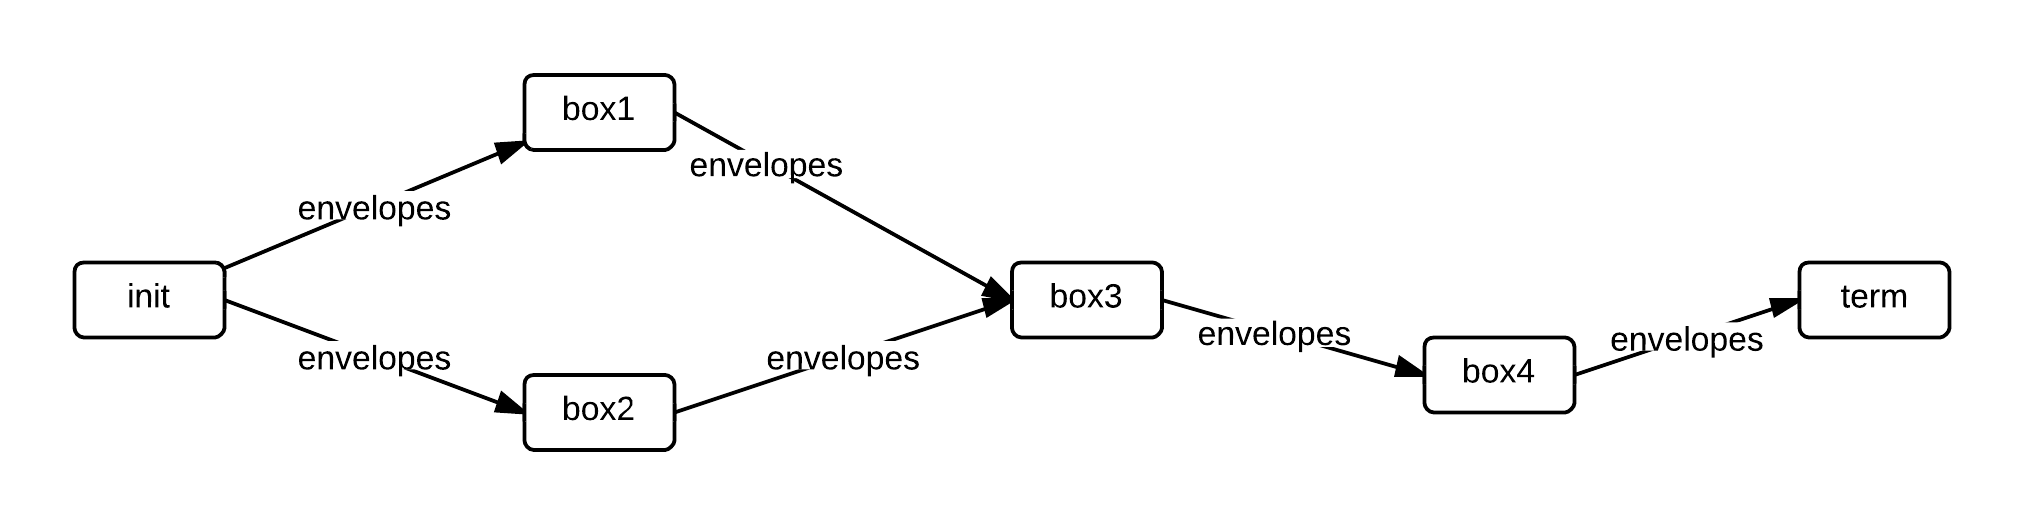
\includegraphics[width=1\textwidth]{bobox}

      \caption{Bobox architecture.}
          \label{fig:bobox}
\end{figure}

Data streams are implemented as streams of data units called envelopes. Envelope structure is displayed in Figure~\ref{fig:envelope}. It consists of sequence of tuples but internally data are stored in columns. Envelope contains sequence of columns and its data is stored in separate list. In order to read all attributes of the $i$-th tuple, we have to access all column lists and read its $i$-th element. Special type of envelope contains a poisoned pill which is sent after all valid data, thus indicating the end of data stream. 

\begin{figure}[h!]
  \centering
    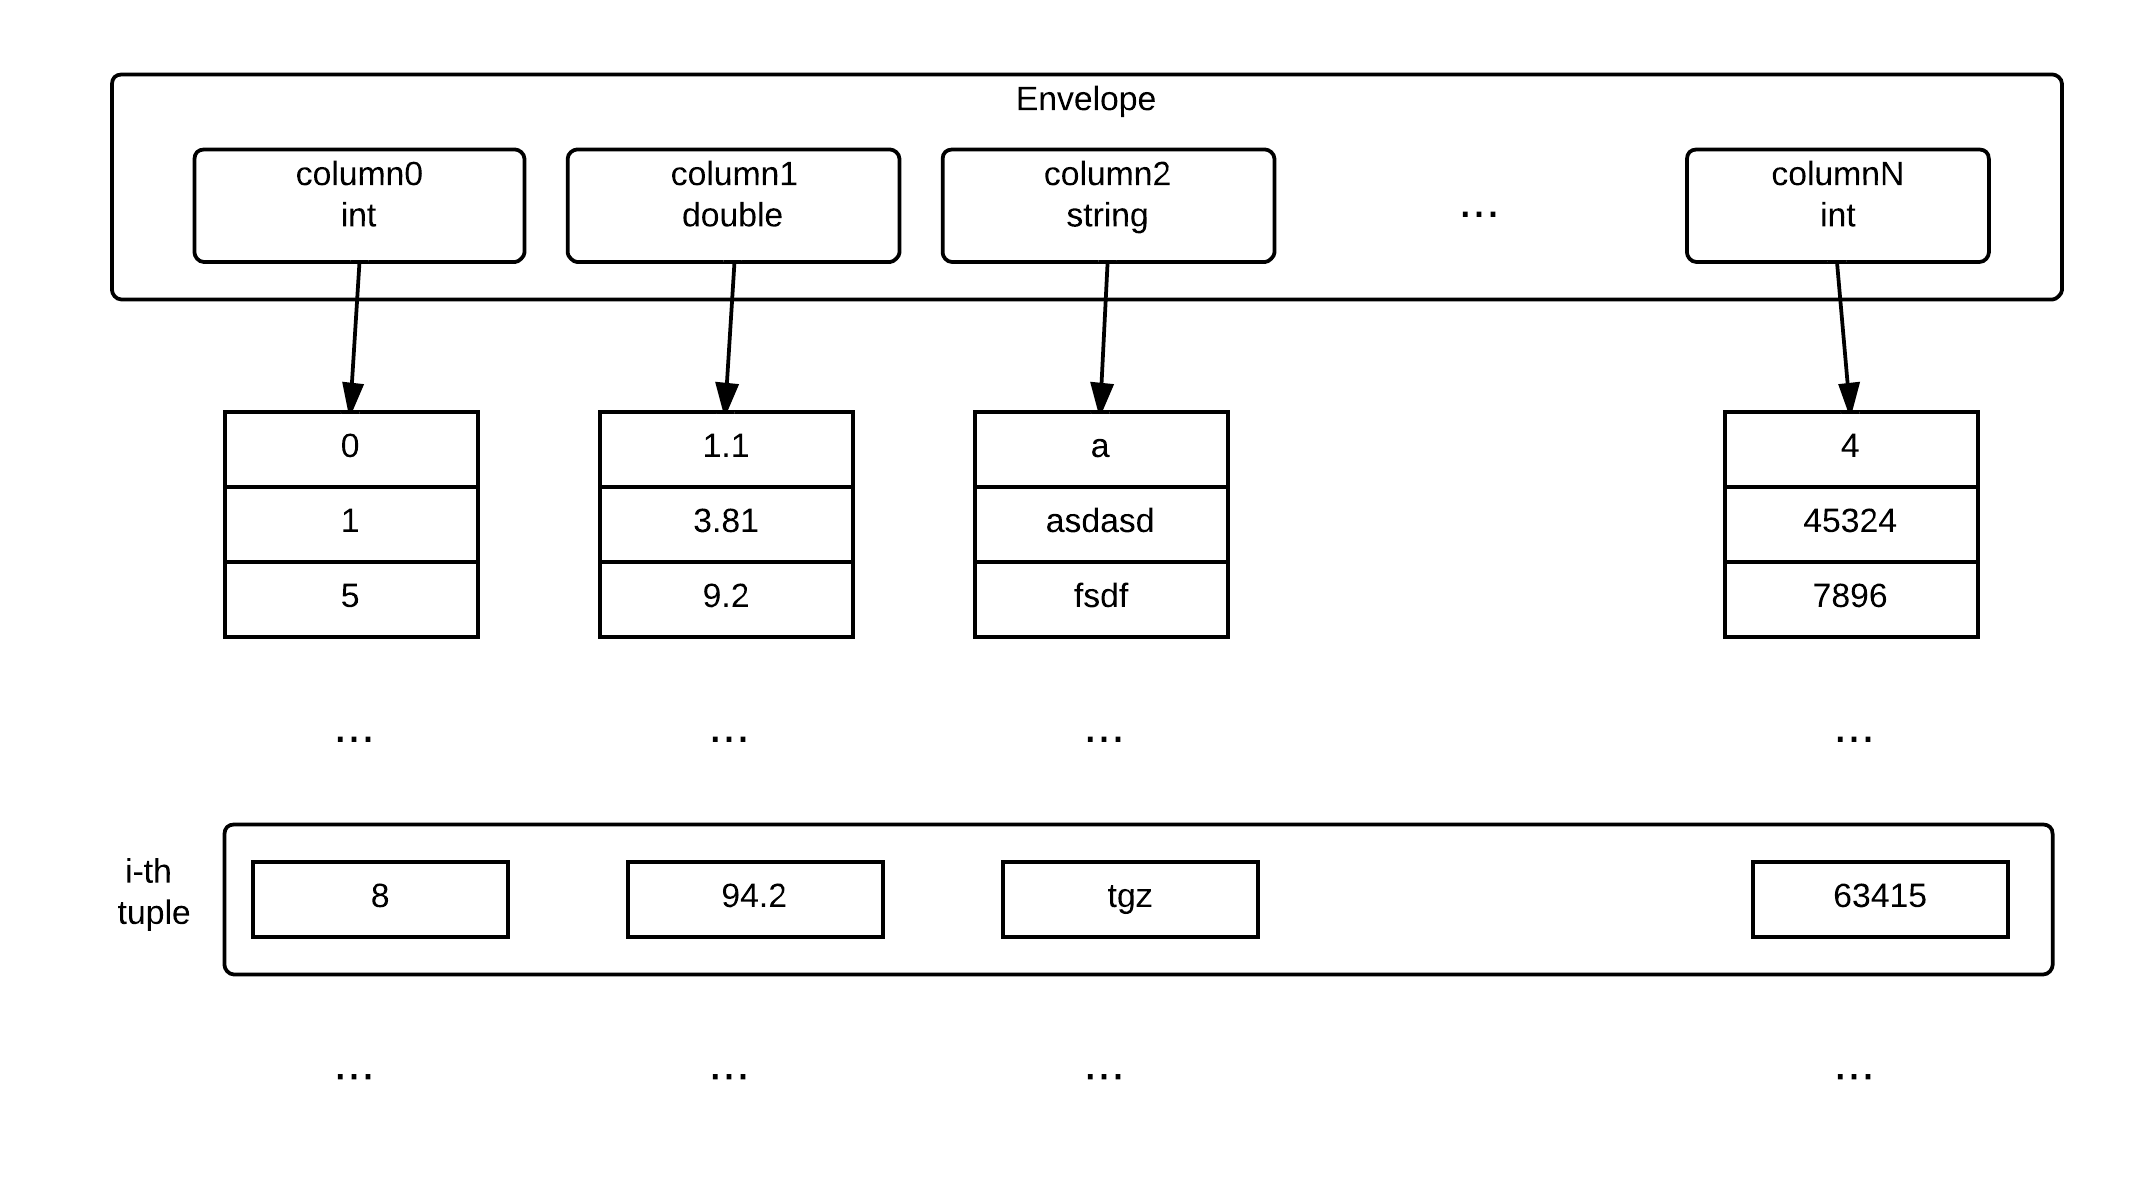
\includegraphics[width=1\textwidth]{envelope}

      \caption{Envelope structure.}
          \label{fig:envelope}
\end{figure}
There are two special boxes, which have to be in every execution plan:
\begin{itemize}


\item $init$ - first box in topological order indicating starting box of execution plan.

\item $term$ - last box in topological order indicating that plan has been completely evaluated.

\end{itemize}

Evaluation starts with scheduling $init$ box, which sends poisoned pills to all of its output boxes that will be scheduled. They can read data from the hard drive or network, process it and send it to other boxes for further processing. Other boxes usually receive data in envelopes in their inputs. Box $term$ waits to receive for its every input to receive poisoned pill and then 
The evaluation ends when the box $term$ receives poisoned pill from each of its inputs.

\section{Bobolang}
Syntax and semantics of Bobolang language is explained in this section. The work Falt et al.~\cite{bobolang} served as source of information for this text.

Bobolang is a formal description language for Bobox execution plan. Bobox environment provides implementation of basic operators (boxes). Bobolang allows programmer to choose which boxes to use, what type of envelopes are passed between boxes and how the boxes are interconnected. 

We can define whole execution plan using operator \verb|main| with empty input and output. An example of complete Bobolang plan:

\begin{verbatim}
operator main()->()
{
    source()->(int) src;
    process(int)->(int,int,int) proc;
    sink(int,int,int)->() sink;

    input -> src -> proc; 
    proc -> sink;
    sink -> output;
}
\end{verbatim}

In the first part, we declare operators and define type of input and output. We provide identifier for every declared operator. Second part specifies connection between declared operators. Code \verb|op1 -> op2| indicates that output of \verb|op1| is connected to input of operator \verb|op2|. In this case, the output type of \verb|op1| has to be equal to the input type of \verb|op2|. Bobolang syntax also allows to create chains of operators like \verb|op1 -> op2 -> op3| with following semantics: \verb|op1 -> op2| and \verb|op2 -> op3|. 

There are explicitly defined operators called \verb|input| and \verb|output|. The line \verb|input -> src;| means that input of the operator \verb|main| is connected to the output of operator \verb|src|.

Bobolang also allows to declare operators with empty input or output with the type \verb|()| meaning that they do not transfer any data. These operators transfer only envelopes containing poisoned pills. The box starts working after receiving poisoned pill. Sending the pill means that all data has been processed and the work is done.


 Structure of example execution plan can be seen in Figure~\ref{fig:exampleplan}. Operators \verb|init| and \verb|term| are added automatically. Operator \verb|init| sends poisoned pill to \verb|source|, which can read data from hard drive or network. Data is sent to the box \verb|process|. Operator \verb|sink| stores data and sends poisoned pill to the box \verb|term| and the computation ends.
\begin{figure}[h!]
  \centering

    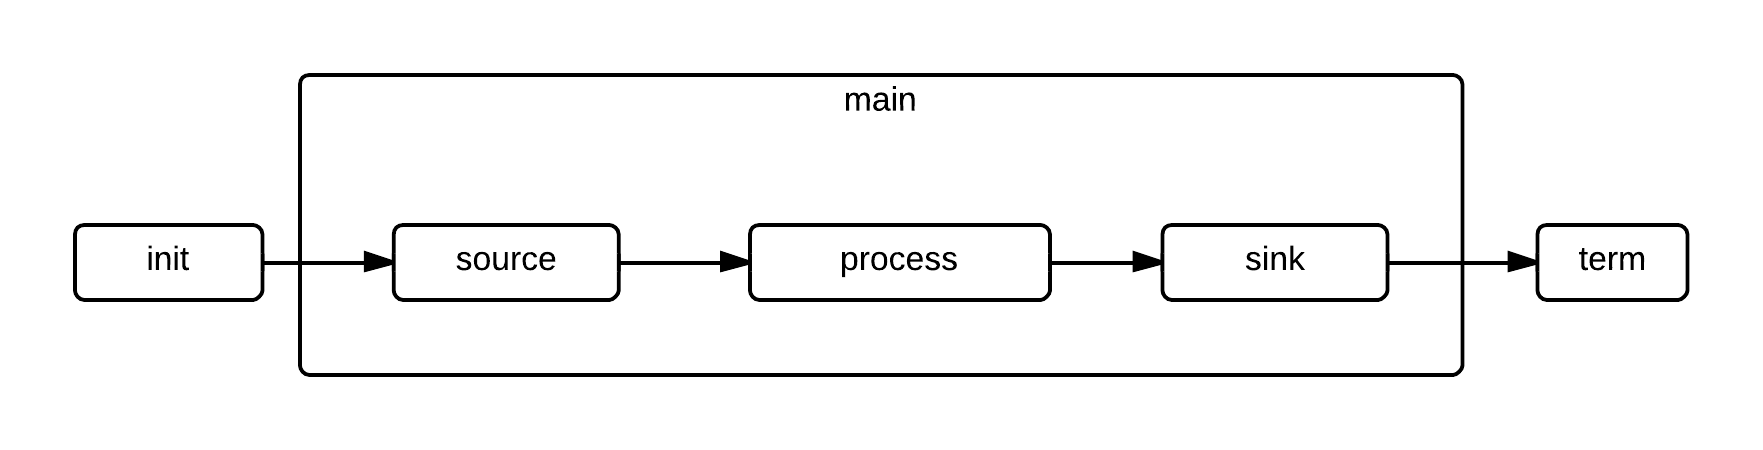
\includegraphics[width=1\textwidth]{exampleplan}
    
      \caption{Example of execution plan.}
        \label{fig:exampleplan}
\end{figure}




